\documentclass[12pt,a4paper]{jbook}
\usepackage{mm-thesis}
\usepackage[dvipdfmx]{graphicx}
\usepackage{cite}
\usepackage{comment}
\usepackage{docmute}
\usepackage{color}
\usepackage{moreverb}
\usepackage{listings}
\usepackage{ascmac}
%\usepackage{amsmath}
%\usepackage{amsthm}
%\usepackage{amsfonts}

\lstset{
	%枠外での自動改行
 	breaklines = true,
 	%標準の書体
 	basicstyle = {\small},
 	%枠 "t"は上に線を記載, "T"は上に二重線を記載
	%他オプション:leftline,topline,bottomline,lines,single,shadowbox
 	frame = TB,
 	%タブの大きさ
 	tabsize = 2,
 	%キャプションの場所("tb"ならば上下両方に記載)
 	captionpos = t,
 	%行番号の位置
 	numbers = left,
 	%自動改行後のインデント量(デフォルトでは20[pt])	
 	breakindent = 30pt,
	%左右の位置調整 	
 	xleftmargin=30pt,
 	xrightmargin=30pt,
	%プログラム言語(複数の言語に対応,C,C++も可)
 	%language = Python, 	
 	%背景色と透過度
 	%backgroundcolor={\color[gray]{.90}},
 	%コメントの書体
 	%commentstyle = {\itshape \color[cmyk]{1,0.4,1,0}},
 	%関数名等の色の設定
 	%classoffset = 0,
 	%キーワード(int, ifなど)の書体
 	%keywordstyle = {\bfseries \color[cmyk]{0,1,0,0}},
 	%表示する文字の書体
 	%stringstyle = {\ttfamily \color[rgb]{0,0,1}},
 	%frameまでの間隔(行番号とプログラムの間)
 	%framesep = 5pt,
 	%行番号の間隔
 	%stepnumber = 1,
	%行番号の書体
 	%numberstyle = \tiny,
}
\renewcommand{\lstlistingname}{Code}
\begin{document}
\newpage

\chapter{提案モデル}
この章では、\ref{sec:ProposedModel-TemporalLogic}章で述べた記述法の応用例として、キャッシュを実装したウェブセキュリティモデルを提案する。

\section{概要}
本研究は基礎モデルで包括されていないウェブの要素としてキャッシュに注目する。
\ref{sec:bcpattack}節に述べた通りキャッシュを利用する攻撃が数多く存在しており、また、キャッシュは一般的なユーザにも利用される。
したがって、キャッシュに関連した脆弱性はウェブの利用者の多くに多大な影響を与えるため、ウェブの安全性を解析する上で不可欠な要素である。
本研究では、キャッシュを包括するウェブセキュリティモデルを提案し、\ref{sec:ProposedModel-TemporalLogic}節で述べた記述法を用いて提案モデルを実装する。

\section{提案モデルの能力}
\label{sec:ProposedModel-Power}
提案モデルは基礎モデルを基に作成する。
基礎モデルの能力は\ref{sec:based-model-power}節で述べており、以下に基礎モデルからの提案モデルでの変更点を各項目ごとに記述する。

\subsection{対象のシステムの構造と動作}
提案モデルでは、キャッシュの動作を包括することを目標とする。
しかし、キャッシュの動作を表現するには中継者やヘッダなど、基礎モデルで包括している項目では不足している要素がある。
したがって、提案モデルにはキャッシュの動作に加えて、その動作に使用されるキャッシュ以外の要素についても追加する。
以下に追加する要素を順に述べる。

\subsubsection{キャッシュの動作}
キャッシュはクライアント、サーバ、中継者のいずれかに属し、\ref{sec:cache}節で述べた「格納」、「再利用」、「検証」という三つの基本動作が可能である。
また、これらのキャッシュの動作はヘッダによって主に制御される。

\subsubsection{中継者}
中継者はクライアントやサーバとは異なるHTTPを構成する第三の要素であり、クライアントとサーバの通信経路上に存在する。
HTTP/1.1において、中継者は「プロキシ」、「ゲートウェイ」、「トンネル」の三種類が存在するが、これらのうちトンネルのみキャッシュを搭載しない。
したがって、キャッシュに注目する提案モデルはプロキシとゲートウェイのみを包括する。

まず、中継者は独自にリクエストやレスポンスを生成することはなく、取得したリクエストやレスポンスの回送を主に行う。
しかし、キャッシュを用いた場合にのみ、リクエストをサーバに送信しレスポンスを得ることなく、キャッシュの再利用をもってリクエストに応答することができる。
また、プロキシとゲートウェイはその通信内容の編集が可能である。

\subsubsection{HTTPヘッダ}
基礎モデルに含まれるヘッダではキャッシュの動作の表現に不十分であるため、表\ref{tb:ProposedModel-Headers}に挙げるヘッダを新たに追加する。

\begin{table}[htb]
\centering
\caption{提案モデルで新たに包括するヘッダ}
\label{tb:ProposedModel-Headers}
\begin{tabular}{lll}
\hline
ヘッダ名 & 用途 & 関連するキャッシュの動作 \\
\hline
if-modified-since & 条件付きリクエストに使用 & 検証 \\
if-none-match & 条件付きリクエストに使用 & 検証 \\
etag & レスポンス内のコンテンツの固有値 & 検証 \\
last-modified & レスポンス内のコンテンツの最終更新日 & 検証 \\
age & レスポンスの経過時間 & 格納・再利用 \\
cache-control & キャッシュの動作全般を制御 & 格納・再利用・検証 \\
date & レスポンスの生成時刻 & 格納・再利用 \\
expire & レスポンスの有効期限 & 格納・再利用 \\
\hline
\end{tabular}
\end{table}

また、表\ref{tb:ProposedModel-Headers}内のcache-controlヘッダはオプションによってキャッシュの動作を指定するため、そのオプションを付加可能とする。
利用可能なオプションを表\ref{tb:CacheControlOption}に挙げる。

\begin{table}[htb]
\centering
\caption{利用可能なcache-controlヘッダのオプション}
\label{tb:CacheControlOption}
\begin{tabular}{ll}
\hline
オプション名 & 用途 \\
\hline
max-age & レスポンスの有効期限を設定 \\
smax-age & 共有キャッシュでの有効期限を設定(その他の設定より優先) \\
no-cache & 検証無しに再利用できない \\
no-store & そのレスポンスを格納を禁止 \\
no-transform & コンテンツの編集を禁止 \\
max-stale & 期限切れである場合に許容できる時間 \\
min-fresh & 有効期限まで最低残り時間 \\
only-if-cached & キャッシュの再利用でのみ応答 \\
must-revalidate & 有効期限切れである場合、検証無しに再利用できない \\
proxy-revalidate & must-revalidateと同じ(個人キャッシュ以外で有効) \\
public & 共有キャッシュに格納してよい \\
private & 個人キャッシュに格納してよい \\
\hline
\end{tabular}
\end{table}

\subsubsection{ブラウザ}
基礎モデルでは表現の単純化のため、「ブラウザのメモリ領域は書き込みのみ可能」という制限がある。
しかし、この制限下ではキャッシュ内の格納レスポンスの削除や検証といった動作を実行することができず、キャッシュの動作を十分に表現することができない。
本研究で提案する時相論理の記述法を用いればレスポンスの削除といった動作を容易に表現できるため、提案モデルではこの制限を取り除く。

\subsection{脅威モデル}
提案モデルの脅威モデルは基礎モデルのものを継承している。
すなわち、三種類の攻撃者とユーザのふるまいを脅威モデルとして設定し、攻撃者にキャッシュと中継者に関する攻撃の能力を新たに付与する。
以下に、三種類の攻撃者それぞれに付与する能力を示す。

\begin{itemize}
\item Web Attacker\\
Web Attackerは複数の中継者を所有することができる。
しかし、その通信内容の編集や通信の遮断をすることはできず、内容をそのままに回送することのみ可能とする。
ただし、暗号化されていない場合、その通信内容を盗聴することは可能とする。
また、保有するクライアント、サーバ、中継者にキャッシュを搭載し、仕様通りに運用できる。
\item Network Attacker\\
Network Attackerは上記のWeb Attackerの能力を全て持つ。
これに加えて、中継者を用いた暗号化されていない通信内容の改ざんと、通信の遮断は可能とする。
\item Gadget Attacker\\
Gadget Attackerは中継者とキャッシュに関する能力は上記のNetwork Attackerと同様の能力を持つ。
\end{itemize}

また、正当なユーザのふるまいに対する制限に特に変更は加えない。

\subsection{安全性要件}
基礎モデルには二つの安全性要件が設定されており、これらの変更はない。
しかし、Security Invariantsにおける「ウェブの各構成要素」という文言にキャッシュや中継者が含まれることとなる。

\section{キャッシュの実装}
\ref{sec:ProposedModel-Power}節で述べた提案モデルの能力を基に、時相論理を用いてキャッシュを表現する。

\subsection{キャッシュクラスの作成}
キャッシュを表すクラスをCode\ref{code:CacheClass}のように記述する。
抽象クラスとしてCacheクラスを定義し、個人キャッシュを表すPrivateCacheクラス、共有キャッシュを表すPublicCacheクラスを定義する。
また、CacheクラスにはCode\ref{code:LimitedCacheClass}に記述する制限を付与する。
付与される制限は以下の二点である。
\begin{itemize}
\item どのネットワーク上の端末にも属さないキャッシュは存在しない(1-4行目)
\item 個人キャッシュはクライアントに属し、共有キャッシュはサーバ、もしくは中継者に属する(6-9行目)
\end{itemize}

\begin{lstlisting}[caption=Cacheクラス, label=code:CacheClass]
abstract sig Cache{}
sig PrivateCache extends Cache{}
sig PublicCache extends Cache{}
\end{lstlisting}

\begin{lstlisting}[caption=Cacheクラスの制限, label=code:LimitedCacheClass]
fact noOrphanedCaches {
	all c:Cache |
		one e:NetworkEndpoint | c = e.cache
}

fact PublicAndPrivate{
	all pri:PrivateCache | pri in HTTPClient.cache
	all pub:PublicCache | (pub in HTTPServer.cache) or (pub in HTTPIntermediary.cache)
}
\end{lstlisting}

また、キャッシュを搭載するため、Code\ref{code:EndPoint}のように、構成要素のクラスを変更する。
HTTPにおけるクライアント、サーバ、中継者を包括するHTTPConfirmistクラスにCacheクラスを追加する。
また、このとき各端末は多くとも一台のキャッシュしか保有することができないものとする。
\begin{lstlisting}[caption=HTTPを利用するウェブの構成要素, label=code:EndPoint]
abstract sig HTTPConformist extends NetworkEndpoint{cache : lone Cache}
\end{lstlisting}

\subsection{キャッシュの状態を表すクラス}
\label{sec:CacheClass}
Code\ref{code:CacheStateClass}のように、時間軸上の各時点におけるキャッシュの状態を表現するクラスを作成する。
このクラスはStateクラスを継承し、作成した時相論理に関する述語を利用可能な形式とする。
また、この形式を用いるために、「一致要素」と「変化要素」を定義する必要がある。
まず、一致要素について考える。
キャッシュの状態遷移は同一のキャッシュの状態間で発生するため、一致要素はキャッシュとする。
これに従い、23行目のように一致要素を表すEqItemクラスを継承したCacheEqItemクラスを定義し、要素としてCacheクラスを定義する。
一方で、キャッシュ内の格納レスポンスの変化を表現するために、変化要素は格納レスポンスとする。
したがって、24行目のように変化要素を表すDifItemクラスを継承したCacheDifItemクラスを定義し、要素としてレスポンスの集合を定義する。
これにより、CacheStateクラスはあるキャッシュのある時点での格納レスポンスを表すクラスとして作成される。

また、Code\ref{code:CacheStateClass}の5-22行目には、CacheStateクラスに以下の条件が記される。
これは、HTTP/1.1の仕様に従ったキャッシュの動作を表現したものである。
\begin{itemize}
\item 個人キャッシュの格納レスポンスのヘッダには、cache-controlヘッダのmax-ageオプション、もしくはdateヘッダとexpireヘッダが一つ含まれる
\item 共有キャッシュの格納レスポンスのヘッダには、cache-controlヘッダのmax-ageオプション、s-maxageオプション、dateヘッダとexpireヘッダのいずれかが一つ含まれる
\item キャッシュの格納レスポンスには、必ずageヘッダが一つ含まれる
\end{itemize}

\begin{lstlisting}[caption=キャッシュの状態を表すクラス, label=code:CacheStateClass]
sig CacheState extends State{}{
	eq in CacheEqItem
	dif in CacheDifItem

	eq.cache in PrivateCache implies
        all res:HTTPResponse | res in dif.store implies
                {
                    (one op:Maxage | op in res.headers.options) or
                    (one d:DateHeader, e:ExpiresHeader | d in res.headers and e in res.headers)
                }

    eq.cache in PublicCache implies
        all res:HTTPResponse | res in dif.store implies
                {
                    (one op:Maxage | op in res.headers.options) or
                    (one op:SMaxage | op in res.headers.options) or
                    (one d:DateHeader, e:ExpiresHeader | d in res.headers and e in res.headers)
                }

    all res:HTTPResponse | res in dif.store implies
        one h:AgeHeader | h in res.headers
}
sig CacheEqItem extends EqItem{cache: one Cache}
sig CacheDifItem extends DifItem{store: set HTTPResponse}
\end{lstlisting}

\color{red}
さらに、これらに加えてCacheState、StateTransactionクラスにはCode\ref{code:LimitedCacheStateClass}に記す条件を付与する。
これらは、モデルをAlloy上で実装する際に必要となる項目である。
まず、1-4行目では同一内容の状態クラスのインスタンスが複数存在しないことを表している。
もし、同一内容のインスタンスが複数存在することを許した場合、単純なインスタンスの比較によってのみでは状態が変化したかどうかを判定できない。
この制限は状態変化の比較を容易にする。
また、10-14行目では、キャッシュが搭載されている端末が通信を行った場合に、そのキャッシュの状態が必ず表現されることを表している。
この記述により、通信が行われた場合にはそのリクエストとレスポンス時点での状態がCacheStateクラスのインスタンスとして必ず表現され、時間軸全体を通して変化を捉えることが可能になる。
\color{black}
\begin{lstlisting}[caption=CacheStateクラスの制限, label=code:LimitedCacheStateClass]
fact noMultipleItems{
	no disj i,i':CacheEqItem | i.cache = i'.cache
	no disj i,i':CacheDifItem | i.store = i'.store
}

fact CacheInTransaction{
	all tr:HTTPTransaction |
		(some tr.request.(from + to).cache implies tr in StateTransaction)

	all str:StateTransaction |{
		str.beforeState.eq.cache = str.request.(from + to).cache
		some str.(request + re_res) implies str.afterState.eq.cache = str.beforeState.eq.cache
	}
}
\end{lstlisting}

\color{red}
\subsection{キャッシュの動作}
\ref{sec:CacheClass}節で定義したCacheStateクラスを用いて、キャッシュの動作を記述する。

\subsubsection{レスポンスの格納と削除}
提案モデルにおいて、キャッシュにおけるレスポンスの格納と削除は以下のように動作するものとする。

\begin{itembox}[l]{レスポンスの格納}
キャッシュは、そのキャッシュが存在する端末が送受信したレスポンスを格納できる。
そのタイミングは、格納レスポンスを送受信したタイミングとする。
また、格納レスポンスは格納することのできる条件をすべて満たしているものとする。
\end{itembox}

\begin{itembox}[l]{レスポンスの削除}
キャッシュは任意のタイミングで、格納されているレスポンスをキャッシュ内から削除できる。
\end{itembox}

上記で定めたレスポンスの格納と削除は図\ref{fig:ProposedModel-ResponseStoreDelete}のように、二状態間の状態変化として表現する。
まず、レスポンスの格納はレスポンス時のキャッシュの状態において、格納レスポンスにそのレスポンスを追加することで表現できる。
これは、図\ref{fig:ProposedModel-ResponseStoreDelete}内のCacheState0と1における状態変化にあたる。
CacheState0は変化要素としてCacheDifItem0を持ち、CacheState1はCacheDifItem1を持つ。
そして、CacheDifItem0は格納レスポンスの集合が空集合であり、CacheDifItem1は格納レスポンスの集合にResponse0を持つ。
これは、StateTransaction0におけるレスポンスがResponse0であり、レスポンス時にそれがCache0に格納されたことを表す。
また、レスポンスの削除は前状態における格納レスポンスの一部を次状態に引き継がないことで表現する。
これは、図\ref{fig:ProposedModel-ResponseStoreDelete}内のCacheState1と2における状態変化にあたる。
この場合、CacheState2は変化要素としてCacheDifItem0を持つため、上述の格納の場合と状態変化が逆になる。
つまり、CacheState1の時点でCache0が格納していたResponse0を、CacheState2の時点では削除していることを表している。

\begin{figure}[htb]
\centering
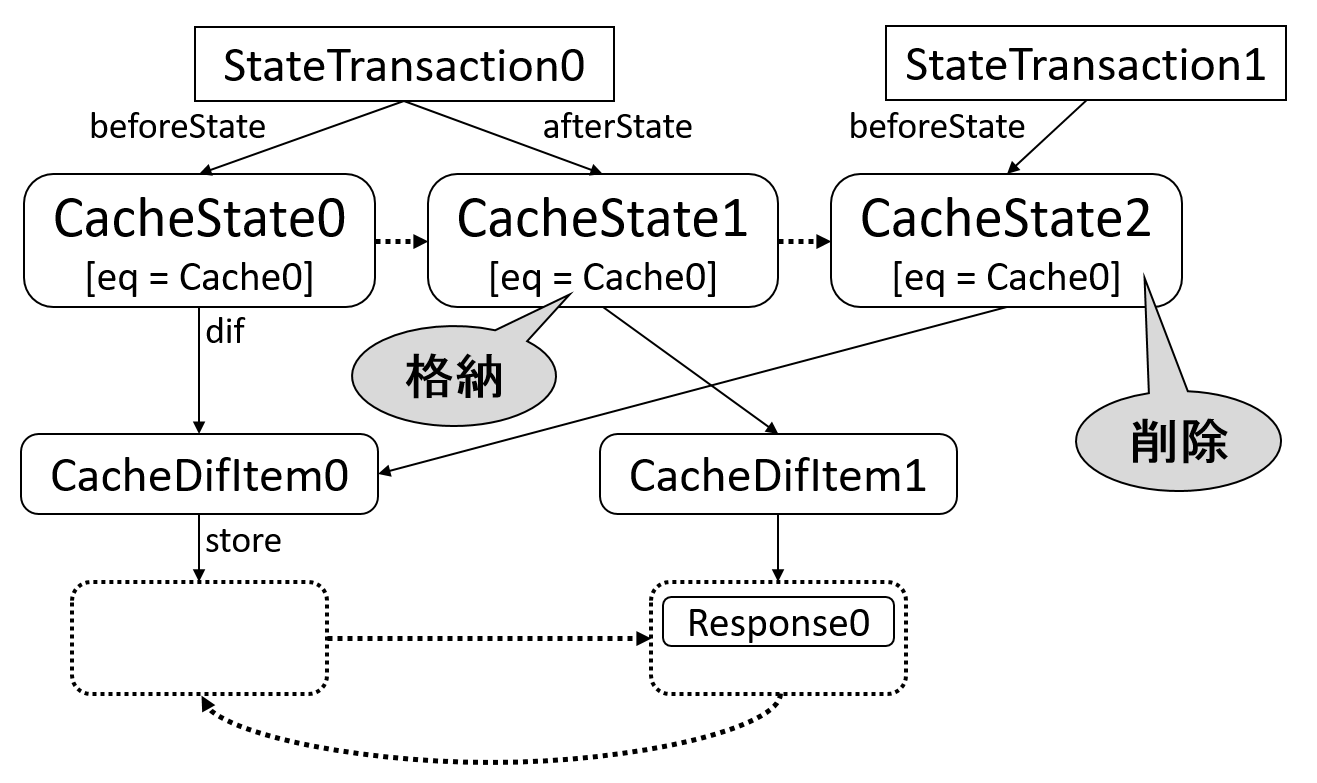
\includegraphics[width=450pt]{./fig/ProposedModel-ResponseStoreDelete.eps}
\caption{キャッシュの格納と削除の表現}
\label{fig:ProposedModel-ResponseStoreDelete}
\end{figure}

また、以上の内容を提案モデルではCode\ref{code:StoreResponse}のように実装している。
格納と削除は主に6-10行目で表されており、ある状態postがリクエスト時の状態である場合は、postの格納レスポンスの集合はpostの前状態であるpreの格納レスポンスの集合の部分集合となる。
この二状態の関係を部分集合とすることで、前状態の格納レスポンスの一部がなくなることを容認し、削除の動作を表現できている。
また、ある状態postがレスポンス時の状態である場合は、上述の削除に加え、格納が行われている可能性がある。
したがって、postの格納レスポンスの集合をpreの格納レスポンスに、そのトランザクションでのレスポンスを加えた集合の部分集合とする。
これにより、削除に加え、レスポンス時における格納を表現できている。
ただしこの既述のみでは各時点でのキャッシュの状態はその前状態に依存することになり、初期状態が無条件となる。
実際には、この場合の初期状態とはウェブ上における様々な通信が行われる前の状態を示すため、初期状態でキャッシュにレスポンスが格納されていることはない。
したがって、初期状態の格納レスポンスの集合を空集合とする制限を、2-4行目で記述している。

\begin{lstlisting}[caption=レスポンスの格納と削除の表現, label=code:StoreResponse]
fact flowCacheState{
	all cs:CacheState |
		FirstState[cs] implies
			no cs.dif.store

	all pre, post:CacheState, str:StateTransaction |
		JustBeforeState[pre, post, str] implies {
			post in str.beforeState implies post.dif.store in pre.dif.store
			post in str.afterState implies post.dif.store in (pre.dif.store + str.response)
		}
}
\end{lstlisting}

\subsubsection{レスポンスの再利用}
提案モデルにおいて、キャッシュによるレスポンスの再利用は以下の動作を示す。

\begin{itembox}[l]{レスポンスの再利用}
キャッシュは、そのキャッシュが存在する端末が送受信するリクエストに対してキャッシュ内の格納レスポンスで応答できる場合、そのレスポンスを用いて応答することができる。
ここで、リクエストの送信者が自身のキャッシュで再利用を行う場合、リクエストは実際はネットワーク上に発信されない。
\end{itembox}

上記で定めたレスポンスの再利用は、提案モデル内では本来発生するレスポンスの代わりとなって発生する。
したがって、既存モデルにおいてレスポンスを表すHTTPResponseクラスと同列に、CacheReuseクラスを定義する(Code\ref{code:CacheReuseClass}参照)。
HTTPResponseクラスはHTTPプロトコル上のイベントを表すHTTPEventクラスを継承しているため、CacheReuseクラスもHTTPEventクラスを継承する。
そして、CacheReuseクラスにある一つのレスポンスを関連付けることで、どのレスポンスを再利用したかを表現できる(5行目)。
また、HTTPEventクラスにおいて、どの端末からどの端末に対するイベントであるかは定義されており、これを利用することで再利用したレスポンスの送信元と送信先を表現する。
しかし、HTTPEventクラスでは送信元と送信先の他に、そのイベントに含まれるヘッダとボディが定義されている。
実際のレスポンスの再利用では、送信されるのは再利用するレスポンスのヘッダとボディであり、それは上記のレスポンスとの関連付け(5行目)で表現されているためこの二項目は不必要である。
したがって、7,8行目のように、CacheReuseクラスのヘッダとボディは空集合とする。

\begin{lstlisting}[caption=CacheReuseクラス, label=code:CacheReuseClass]
sig HTTPResponse extends HTTPEvent {
	statusCode: one Status
}
sig CacheReuse extends NetworkEvent{
	target: one HTTPResponse
}{
	no headers
	no body
}
\end{lstlisting}

上記で定義したCacheReuseクラスを用いて再利用を表現するため、Code\ref{code:happenCacheReuse}のように実際のキャッシュの動作に基づいた条件を付加する。
付加した条件は以下の通りである。
\begin{itemize}
\item 再利用するレスポンスの送信先は、その再利用を発生させたリクエストの送信元である(5行目)
\item 再利用するレスポンスの送信元は、その再利用を発生させたリクエストの送信元、もしくは、送信先である(6行目)
\item 再利用を行うキャッシュの再利用直前の状態において、再利用するレスポンスが格納レスポンスに含まれている(8-13行目)
\item 再利用するレスポンスと、その再利用を発生させたリクエストが表すURIが一致している
\end{itemize}

\begin{lstlisting}[caption=CacheReuseの発生条件, label=code:happenCacheReuse]
fact happenCacheReuse{
	all reuse:CacheReuse | one str:StateTransaction |
		{
			str.re_res = reuse
			reuse.to = str.request.from
			reuse.from in str.request.(from + to)

			some pre, post:CacheState |
				(post in str.afterState and JustBeforeState[pre, post, str]) implies
					{
						reuse.target in pre.dif.store
						reuse.from.cache = pre.eq.cache
					}

			reuse.target.uri = str.request.uri
		}
}
\end{lstlisting}

上記の条件の二点目において、再利用レスポンスの送信元がリクエストの送信元となる場合を認めるのは、そのリクエストを送信した端末のキャッシュによるレスポンスの再利用を想定するためである。
例えば、図\ref{fig:BrowserCacheReuse}のようなブラウザキャッシュによるレスポンスの再利用である。
図\ref{fig:BrowserCacheReuse}はブラウザがサーバにリクエストを送信する際に、ブラウザのキャッシュ内に既に格納されているレスポンスResponse0を再利用する流れを表している。
このような場合には、CacheReuse0のfromとtoは同一のBrowser0を指すことになる。
このような状況を想定し二点目の条件を設定している。

\begin{figure}[htb]
\centering
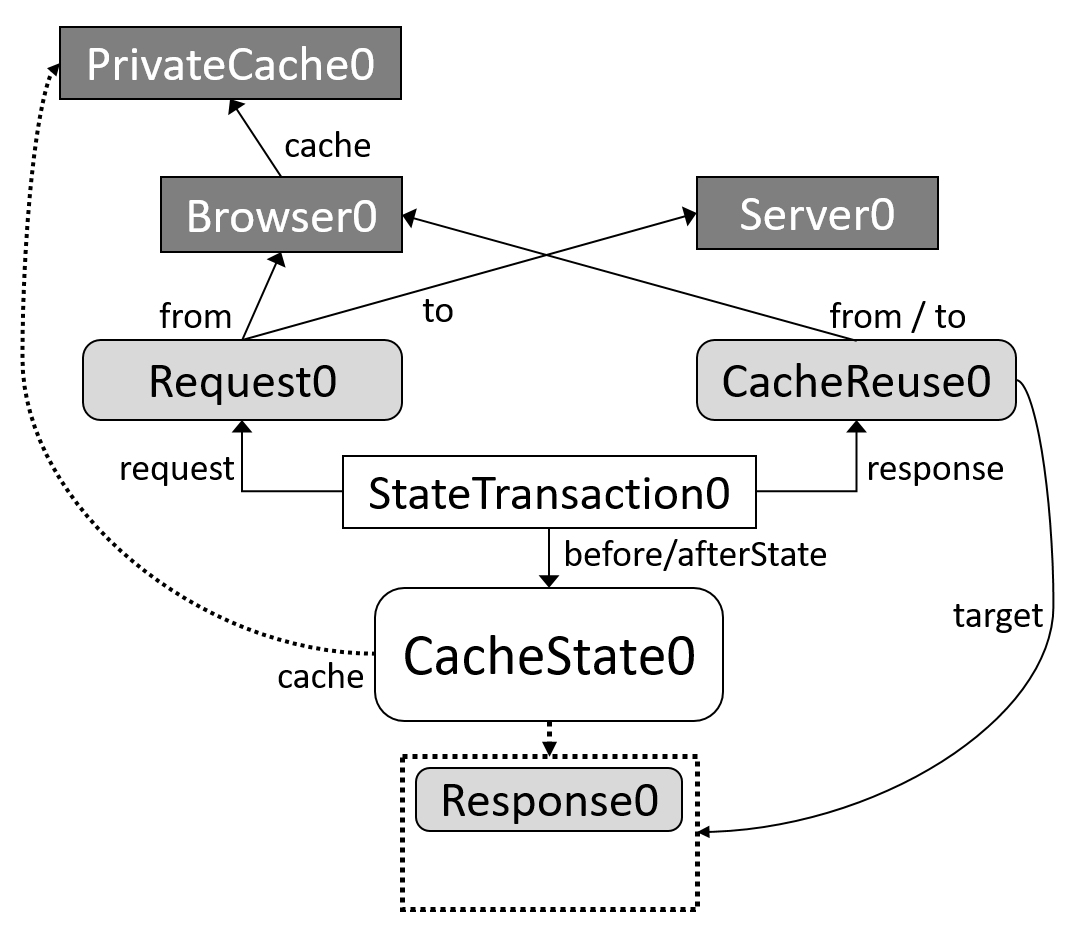
\includegraphics[width=400pt]{./fig/BrowserCacheReuse.eps}
\caption{ブラウザキャッシュでのレスポンスの再利用の一例}
\label{fig:BrowserCacheReuse}
\end{figure}

\subsubsection{格納レスポンスの検証}
提案モデルにおいて、キャッシュによる格納レスポンスの検証を以下のように定義する。

\begin{itembox}[l]{格納レスポンスの検証}
格納レスポンスは、格納レスポンスが再利用可能であるかを判定するために、条件付きリクエストを送信しオリジンサーバに問い合わせを行う。
条件付きリクエストは、if-modified-sinceヘッダかif-none-matchヘッダのいずれかが含まれるリクエストのことを指す。
これらのヘッダで送信される値を用いることで、オリジンサーバは格納レスポンスが最新のものと同一であるかを判定でき、再利用の可否をレスポンスで送信する。
このレスポンスの状態コードは、検証が正常に終了した場合304か200となる。
\begin{itemize}
\item 再利用可能である場合 \\
レスポンスの状態コードは304となり、そのヘッダやボディの値に関係なくキャッシュは格納レスポンスを再利用できる。
\item 再利用不可である場合 \\
レスポンスの状態コードは200となり、検証動作を発生させた元々のリクエストに対して検証動作の結果として返されるレスポンスを用いて返答する。
またこの場合、格納されていたレスポンスは削除され、検証結果のレスポンスをキャッシュに格納し再利用を行う。
\end{itemize}
また、検証後はどちらの場合も再利用可能なレスポンスの一つを除いて、同一のURIに対するレスポンスはキャッシュ内には存在しない。
\end{itembox}

この動作の実装は以下の二つを表現することで実現できる。
\begin{itemize}
\item レスポンスの再利用が行われている場合に、その再利用レスポンスが検証済みであるかを判定する述語
\item 条件付きリクエストに対するサーバの動作
\end{itemize}

まず、検証済みかを判定する述語checkVerificationをCode\ref{code:checkVerification}に示す。
この述語checkVerificationはStateTransaction(strとする)を入力とする。
述語checkVerificationは、strが再利用によって応答されているトランザクションであり、かつ、strのリクエストと再利用の間に条件付きリクエストを含むトランザクションが成立している場合に真となるように作成し、その論理は以下のように表せる。

\begin{itembox}[l]{述語checkVerification}
入力であるStateTransactionクラスのインスタンスであるstrが再利用を行っており、かつ、以下を満たすStateTranactionのクラスのインスタンスstr'が存在する場合に、本述語は真となる。
\begin{itemize}
\item strとstr'は異なるトランザクションである
\item str'のレスポンスが存在する(通信が正常に完了している)
\item str'のリクエストはstrの後に発生し、str'のレスポンスはstrの再利用より前に発生している
\item str'のリクエストは、strの再利用が行われるキャッシュが属する端末から、再利用するレスポンスの送信元に送信されている
\item strとstr'での要求URIが同一である
\item 検証対象の格納レスポンスにetagヘッダかlast-modifiedヘッダが含まれている
\item 検証対象の格納レスポンスにetagヘッダが含まれている場合、str'のリクエストにif-none-matchヘッダが含まれる
\item 検証対象の格納レスポンスにlast-modifiedヘッダが含まれている場合、str'のリクエストにif-modified-sinceヘッダが含まれる
\end{itemize}
\end{itembox}

\begin{lstlisting}[caption=ある再利用が検証済みか判定する述語, label=code:checkVerification]
pred checkVerification[str:StateTransaction]{
	one str.re_res

	some str':StateTransaction |
	{
		str' != str
		one str'.response

		str'.request.current in str.request.current.*next
		str.re_res.current in str'.response.current.*next

		str'.request.from = str.re_res.from
		str'.request.to = str.re_res.target.from
		str'.request.uri = str.request.uri

		some h:HTTPHeader |{
			h in ETagHeader + LastModifiedHeader
			h in str.re_res.target.headers
		}

		(some h:ETagHeader | h in str.re_res.headers) implies
			(some h:IfNoneMatchHeader | h in str'.request.headers)
		(some h:LastModifiedHeader | h in str.re_res.headers) implies
			(some h:IfModifiedSinceHeader | h in str'.request.headers)
	}
}
\end{lstlisting}

また、条件付きリクエストに関するサーバの動作をCode\ref{code:ConditionalRequestTransaction}に示す。
Code\ref{code:ConditionalRequestTransaction}内で、HTTPTransactionクラスのインスタンスtrが条件付きリクエストである場合、以下を満たす。
\begin{itemize}
\item 検証後に、その検証対象のレスポンスのURIを持つ格納レスポンスは一つとなる(5-14行目)
\item trのレスポンスの状態コードは200か304である(16行目)
\item trのレスポンスの状態コードが200である場合、trのレスポンスはキャッシュに格納される(18-23行目)
\item trのレスポンスの状態コードが304である場合、trのレスポンスはキャッシュに格納されない(25-30行目)
\end{itemize}

\begin{lstlisting}[caption=条件付きリクエストに対するサーバの動作, label=code:ConditionalRequestTransaction]
fact ConditionalRequestTransaction{
	all tr:HTTPTransaction |
		(some h:HTTPHeader | h in IfNoneMatchHeader + IfModifiedSinceHeader and h in tr.request.headers) implies
		{
			one res:HTTPResponse |
			{
				res.uri = tr.response.uri
				one cs:CacheState |
				{
					res in cs.dif.store
					cs.eq.cache = tr.request.from.cache
					cs in tr.afterState
				}
			}

			tr.response.statusCode in c200 + c304

			tr.response.statusCode = c200 implies
			{
				all cs:CacheState |
					(cs in tr.afterState and cs.eq.cache = tr.response.to.cache) implies
						tr.response in cs.dif.store
			}

			tr.response.statusCode = c304 implies
			{
				all cs:CacheState |
					(cs in tr.afterState and cs.eq.cache = tr.response.to.cache) implies
						tr.response !in cs.dif.store
			}
		}
}
\end{lstlisting}
\color{black}

\section{中継者の実装}
\color{red}
提案モデルにおいて中継者はHTTP/HTTPSプロトコルで動作し、プロキシとゲートウェイを包括する。
したがって、HTTPに遵守する端末を表すHTTPConfirmistを継承する形で中継者のクラスを宣言する。
また、中継者のクラスを継承し、プロキシとゲートウェイのクラスを宣言する。
これらのクラスは以下のコードで実装される。

\begin{lstlisting}[caption=中継者、プロキシ、ゲートウェイのクラス, label=code:IntermediaryClass]
abstract sig NetworkEndpoint{}
abstract sig HTTPConformist extends NetworkEndpoint{cache : lone Cache}
abstract sig HTTPIntermediary extends HTTPConformist{}
sig HTTPProxy extends HTTPIntermediary{}
sig HTTPGateway extends HTTPIntermediary{}
\end{lstlisting}

基礎モデルの要素も含め、提案モデルでのネットワーク構成要素のクラス関係は図\ref{fig:NetworkComponent}のようになる。

\begin{figure}[htb]
\centering
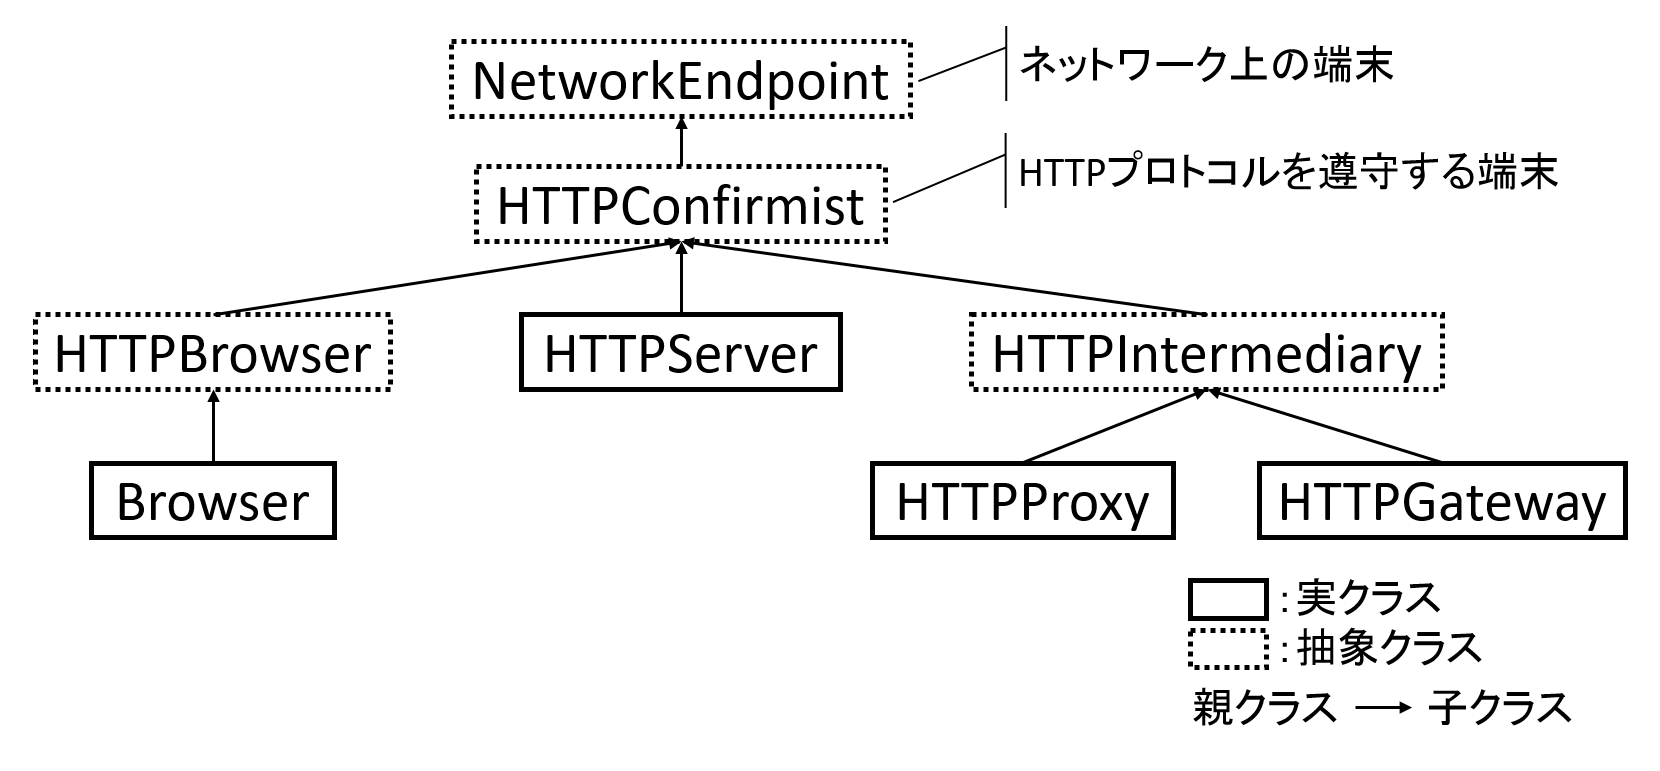
\includegraphics[width=450pt]{./fig/NetworkComponent.eps}
\caption{提案モデルにおけるネットワーク構成要素のクラス関係}
\label{fig:NetworkComponent}
\end{figure}

また、この中継者の動作をCode\ref{code:MoveOfIntermediary}のように記述する。
中継者の動作はリクエストの送信先がHTTPIntermediaryクラスであり、かつ、レスポンスが存在するHTTPTransactionクラスに対する条件として記述する。
このようなHTTPTransactionクラスのインスタンスtrに対して、以下を満たすHTTPTransactionクラスのインスタンスtr'が少なくとも一つ存在する。
\begin{itemize}
\item tr'のリクエストはtrのリクエストの後に発生し、tr'のレスポンスはtrのレスポンスの前に発生する(5,6行目)
\item tr'のリクエストの送信先は、trのリクエストの送信先である中継者である(9行目)
\item trとtr'のリクエストのURIは同一である(10行目)
\item trとtr'のレスポンスのbodyと状態コードは同一である(11,12行目)
\end{itemize}
ただし、上記の動作は正当なユーザに管理された中継者の動作であり、攻撃者が管理する中継者のふるまいはこの限りではない。

\begin{lstlisting}[caption=中継者の動作, label=code:MoveOfIntermediary]
fact MoveOfIntermediary{
	all tr:HTTPTransaction |{
		tr.request.to in HTTPIntermediary and one tr.response implies{
			some tr':HTTPTransaction |{
				tr'.request.current in tr.request.current.*next
				tr.response.current in tr'.response.current.*next

				tr.request.to in WebPrincipal.servers implies{
					tr'.request.from = tr.request.to
					tr'.request.uri = tr.request.uri
					tr.response.body = tr'.response.body
					tr.response.statusCode = tr'.response.statusCode
				}
			}
		}
	}
}
\end{lstlisting}

\color{black}

\section{提案モデルの制限事項}

\end{document}
